%% Layout of a paper figure, filled by scripts/exporters/export_paper_figs.py: every %%PLOTS%% line is replaced by the
%% plots of one axis, in order. Lines starting with %% are dropped from the output.
% Zero-shot classification: (a) average accuracy of every model, (b) Qwen3-32B and Gemma-4-31B.
% Requires pgfplots (compat=1.18), xcolor, graphicx and \usepackage{subcaption}.
% pastelgreen is the green end of the heatmaps' colormap, pastelgreendark its darker counterpart; both are
% global so that the text can name them.
\definecolor{pastelgreen}{RGB}{143,206,143}
\definecolor{pastelgreendark}{RGB}{70,140,70}
\begin{figure}[ht]
\centering
\vspace{-5pt}
\def\plotheight{2.8cm}
\def\barswatch#1#2{\tikz[baseline=0ex]{\fill[#1] (0,0) -- (0,0.2) -- (0.2,0.2) -- cycle; \fill[#2] (0,0) -- (0.2,0) -- (0.2,0.2) -- cycle;}}
\def\curveswatch#1{\tikz[baseline=-0.6ex]\draw[#1, thick, mark=*, mark size=1.5] plot coordinates {(0,0) (0.4,0)};}
\begin{subfigure}[b]{0.47\textwidth}
\centering
\mbox{\barswatch{red!70!black}{pastelgreendark}~{\scriptsize Dropout \&\ Noise}}\hspace{1em}%
\mbox{\barswatch{red!40}{pastelgreen}~{\scriptsize Masking \&\ Jitter}}\\[2pt]
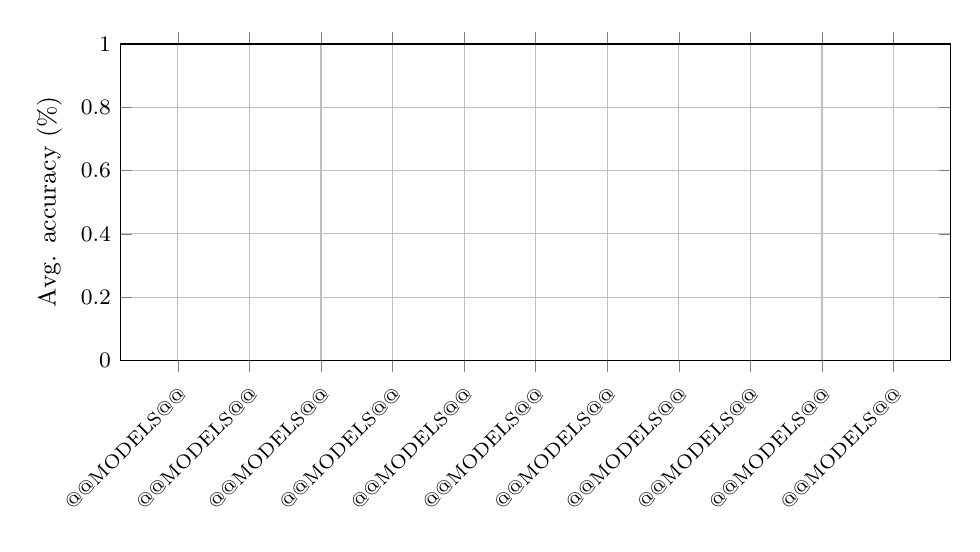
\begin{tikzpicture}
\begin{axis}[
    ybar,
    bar width=4.5pt,
    height=5.6cm,
    width=\linewidth,
    grid=major,
    ylabel={\small Avg. accuracy (\%)},
    ymin=40, ymax=70,
    ytick={40,50,60,70},
    extra y ticks={50},
    extra y tick labels={},
    extra y tick style={grid=major, major grid style={gray, dashed, line width=0.5pt}},
    symbolic x coords={@@MODELS@@},
    xtick={@@MODELS@@},
    tick label style={font=\footnotesize},
    xticklabel style={font=\scriptsize, rotate=45, anchor=north east},
    enlarge x limits=0.08,
]
%%PLOTS%%
\end{axis}
\end{tikzpicture}
\label{fig:zero_shot_average}
\end{subfigure}
\hfill
\begin{subfigure}[b]{0.49\textwidth}
\centering
%% 2.4cm holds the y label, the tick labels and the 0.6cm gap: the block fills the subfigure without scaling its fonts
\edef\plotwidth{\the\dimexpr(\linewidth-2.4cm)/2\relax}
\begin{tabular}[b]{@{}l@{}}
\multicolumn{1}{@{}c@{}}{{\scriptsize \model{qwen32}:}\hspace{0.6em}\mbox{\curveswatch{pastelgreendark}~{\scriptsize Dropout/Noise}}\hspace{0.6em}\mbox{\curveswatch{pastelgreen}~{\scriptsize Masking/Jitter}}}\\[2pt]
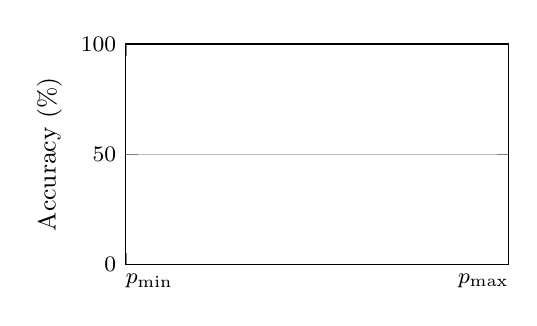
\begin{tikzpicture}[trim axis right]
\begin{axis}[
    height=\plotheight,
    width=\plotwidth,
    scale only axis,
    grid=major,
    ylabel={\small Accuracy (\%)},
    xmin=0, xmax=100,
    xtick={0,100},
    xticklabels={\makebox[0pt][l]{$p_{\min}$},\makebox[0pt][r]{$p_{\max}$}},
    ymin=0.0, ymax=100.0,
    ytick={0,50,100},
    tick label style={font=\footnotesize},
]
%%PLOTS%%
\end{axis}
\end{tikzpicture}%
\hspace{0.6cm}%
\begin{tikzpicture}[trim axis left]
\begin{axis}[
    height=\plotheight,
    width=\plotwidth,
    scale only axis,
    grid=major,
    yticklabels={},
    xmin=0, xmax=100,
    xtick={0,100},
    xticklabels={\makebox[0pt][l]{$\sigma_{\min}$},\makebox[0pt][r]{$\sigma_{\max}$}},
    ymin=0.0, ymax=100.0,
    ytick={0,50,100},
    tick label style={font=\footnotesize},
]
%%PLOTS%%
\end{axis}
\end{tikzpicture}\\[4pt]
\multicolumn{1}{@{}c@{}}{{\scriptsize \model{gemma31}:}\hspace{0.6em}\mbox{\curveswatch{red!70!black}~{\scriptsize Dropout/Noise}}\hspace{0.6em}\mbox{\curveswatch{red!40}~{\scriptsize Masking/Jitter}}}\\[2pt]
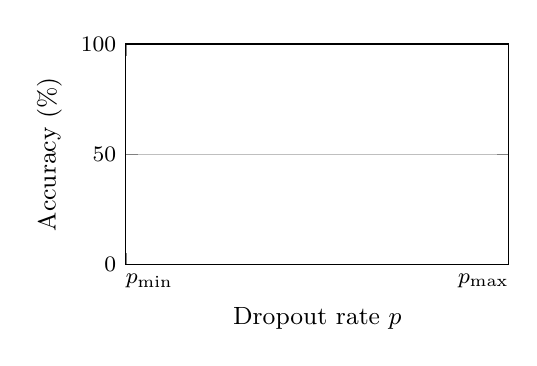
\begin{tikzpicture}[trim axis right]
\begin{axis}[
    height=\plotheight,
    width=\plotwidth,
    scale only axis,
    grid=major,
    xlabel={\small Dropout rate $p$},
    ylabel={\small Accuracy (\%)},
    xmin=0, xmax=100,
    xtick={0,100},
    xticklabels={\makebox[0pt][l]{$p_{\min}$},\makebox[0pt][r]{$p_{\max}$}},
    ymin=0.0, ymax=100.0,
    ytick={0,50,100},
    tick label style={font=\footnotesize},
]
%%PLOTS%%
\end{axis}
\end{tikzpicture}%
\hspace{0.6cm}%
\begin{tikzpicture}[trim axis left]
\begin{axis}[
    height=\plotheight,
    width=\plotwidth,
    scale only axis,
    grid=major,
    xlabel={\small Noise SD $\sigma$},
    yticklabels={},
    xmin=0, xmax=100,
    xtick={0,100},
    xticklabels={\makebox[0pt][l]{$\sigma_{\min}$},\makebox[0pt][r]{$\sigma_{\max}$}},
    ymin=0.0, ymax=100.0,
    ytick={0,50,100},
    tick label style={font=\footnotesize},
]
%%PLOTS%%
\end{axis}
\end{tikzpicture}
\end{tabular}%
\label{fig:zero_shot_detection}
\end{subfigure}
\caption{\small
We apply {dropout} or add {Gaussian noise} to the activations of a target sentence in a prompt, ask \emph{``Did we apply dropout or noise?''}, and report accuracy with the Dropout/Noise labels (dark) and the synonyms Masking/Jitter (light). The average (over dropout and noise samples across strengths) of many models is above chance (\textbf{left}), with \textcolor{pastelgreendark}{two models} increasingly answering \emph{dropout} (or \emph{masking}) when in fact dropout is applied, and likewise for \emph{noise} (or \emph{jitter}) (\textbf{right}).
}
\label{fig:zero_shot_main}
\end{figure}
